\graphicspath{ {02-CoordinateSystems/Figures/} }

\section{Coordinate systems}

\subsection{Laboratory coordinate system}

The origin of the LhARA coordinate system, the ``laboratory coordinate
system'' or ``laboratory reference frame'', is at the position of the
laser focus at the position of the laser-target interaction.
The $z$ axis is horizontal and points along the nominal capture axis,
pointing in the downstream direction, i.e. away from the target.
The $y$ axis points vertically upwards, and the $x$ axis completes a
right-handed orthogonal coordinate system. 

Phase-space coordinates as well as vector and scalar quantities
referred to the laboratory coordinate system will be written without a
suffix. 
Unit vectors along the $x$, $y$ and $z$ axes are $\bm{i}$, $\bm{j}$
and $\bm{k}$ respectively.
The position of the reference particle, its momentum and energy are
described as functions of the distance it has travelled from the origin
of coordinates to its current position.
The distance travelled is defined to be $s$, making the position,
$\bm{r}$, momentum, $\bm{p}$, and energy, $E$, of the particle at
position $s$:
\begin{eqnarray}
  \bm{r} & = & \bm{r}(s)\, ;           \nonumber \\
  \bm{p} & = & \bm{p}(s)\, {\rm ; and} \nonumber \\
      E  & = &     E (s)\, .           \nonumber
\end{eqnarray}
The time, $t$, at which the reference particle is at $s$ is also a
function of $s$:
\begin{eqnarray}
      t  & = & t(s) = \frac{p}{Ec}\, ; \nonumber
\end{eqnarray}
where $p=\left|\bm{p}\right|$ and $c$ is the speed of light.

\subsection{Reference particle local coordinate system}

A coordinate system defined relative to the position of the reference
particle, the ``reference particle local coordinaate'' (RPLC) system,
may be defined using the direction in which the particle is
travelling. 
The position of the particle defines the origin of the RPLC system,
see figure~\ref{fig:RPLC}.
\begin{figure}
  \begin{center}
    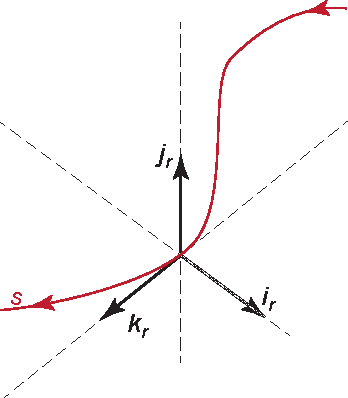
\includegraphics[width=0.55\linewidth]{RPLC.pdf}
  \end{center}
  \caption{
    Reference particle local coordinate system.
    The trajectory of the reference particle is shown as the red line.
    The distance the reference particle has travelled, measured from
    the origin of coordinates in the laboratory frame, is labelled
    $s$.
    The origin of the RPLCs is coincident with the position of the
    reference particle.
    The directions of unit vectors along each of three righthanded,
    orthogonal coordinate axes are shown as black arrows labelled
    $\bm{i}_r$, $\bm{j}_r$, and $\bm{j}_r$. 
  }
  \label{fig:RPLC}
\end{figure}

Phase-space coordinates as well as vector and scalar quantities
referred to the laboratory coordinate system will be written with the
suffix ``$r$''. 
The tangent to the reference particle trajectory at $s$ defines the
$z_r$ axis with unit vector $\bm{k}_r$.
The presence of local electric or magnetic fields may cause the
reference particle's trajectory to curve.
In the neighbourhood of the particle, the curved trajectory may be
described in terms of an arc of a cicle.
The $x_r$ axis (with unit vector $\bm{i}_r$) is then taken to be in
the direction pointing towards the centre of the circle.
The third coordinate axis, $y_r$, is defined to complete the
right-handed orthogonal coordinate system; the unit vector along the
$y_r$ axis being given by $\bm{j}_r = \bm{k}_r \times \bm{i}_r$.

The trajectory of the reference particle will be a straight line as it
traverses a drift space or when the particle's energy is increased (or
decreased) through an electric field applied parallel to its direction
of motion.
In such cases the RPLC axes are taken to coincide with either the
laboratory coordinate system or the RPLC system defined at the exit of
the beam-line element that preceded the drift space or accelating
element.

\subsection{Transforming to and from reference particle local
            coordinates to laboratory coordinates}


